%\section{ Hamiltonian theory}
%\label{sec:theory}
The wave-particle interaction is described by the Hamiltonian on the local cells 
at position $s$ along the dipole field, with phase space characterized by the canonical coordinates $(\xi$, $\Omega)$ in the frame of reference moving with the local resonance
\cite{zheng2024}.
In the Vlasov simulations of  the onset of chorus
\cite{zheng2024,zheng2023b}, we choose the reference frame fixed at the frequency  $\omega_l$ and wave number $k_l$  of the most unstable whistler wave which is excited from the electron temperature anisotropy \cite{gary_1993}. 
Since $\omega_l$ and $k_l$ are constant in time, we refer such reference frame as the static resonance frame. 
The Hamiltonian of resonant electrons  for the onset of chorus is 
\cite{zheng2024}
\begin{equation}\label{eq.H_lab}
    K = \frac{k_l^2\Omega^2}{2} + {\Re}\left(\frac{\omega_b^2}{k_l^2} e^{-\imath \xi} + \frac{\omega_b^2}{k_l^2}\alpha \cdot \xi \right)~,
\end{equation}
where ${\Re}$ denotes taking the real part, 
\begin{equation}\label{eq.alpold}
   \alpha  \simeq \frac{k_l}{\omega_{b}^2}(\mathcal{J} - \frac{\Pi}{2}) \frac{d\omega_{ce}}{ds}~
\end{equation}
is the inhomogeneous parameter,
and 
\begin{equation}
    {\omega_b^2} = k_l^2 a(s,t) \sqrt{2\omega_{ce}\mu(s)}~,
\end{equation}
is the bounce frequency 
with $\mu(s) = \mathcal{J}(s)+\Pi(s)+\Omega$.
Here $\mathcal{J}$ is the canonical momentum associated with the slow-scale motion along the field line
and the parameter $\Pi = v_r/k_l$ is 
from the canonical transformation, 
where  $v_r(s)=(\omega - \omega_{ce})/k_l$ is the resonance velocity. The cyclotron frequency $\omega_{ce}(s)$ 
and 
the parameter $\Pi(s)$
are determined from the background plasma parameters along the dipole field \cite{zheng2024,zheng2023b}, 
as shown in Figs. \ref{fig.aanda}(a) and \ref{fig.aanda}(b).
The  wave envelope of the vector potential $a$ becomes a complex number with an additional phase $\delta \phi$ since the static frame can not exactly follow the real-time resonance. 
The complex wave vector potential $a$ is written as 
\begin{equation}
    a(s,t) = |a(s,t)| \cdot e^{\imath \delta \phi(s,t)}~.
\end{equation}
Therefore, we take the real part in the wave-particle interaction term in the  Hamiltonian Eq. (\ref{eq.H_lab}).
In the Vlasov simulation,
 the wave propagates along the background magnetic field from upstream to the downstream region.
The resonant electrons 
move opposite to the motion of the wave packet.  
The frequency chirping can be seen from Fig. \ref{fig.aanda}(c) where the additional phase $\delta \phi$ results in a modulation on the wave envelope.
The chorus wave is triggered in the source region near the equator and propagates to the downstream where a prominent wave envelope forms in the propagation region, as shown in Fig. \ref{fig.aanda}(d).

\begin{figure}
    \centering
    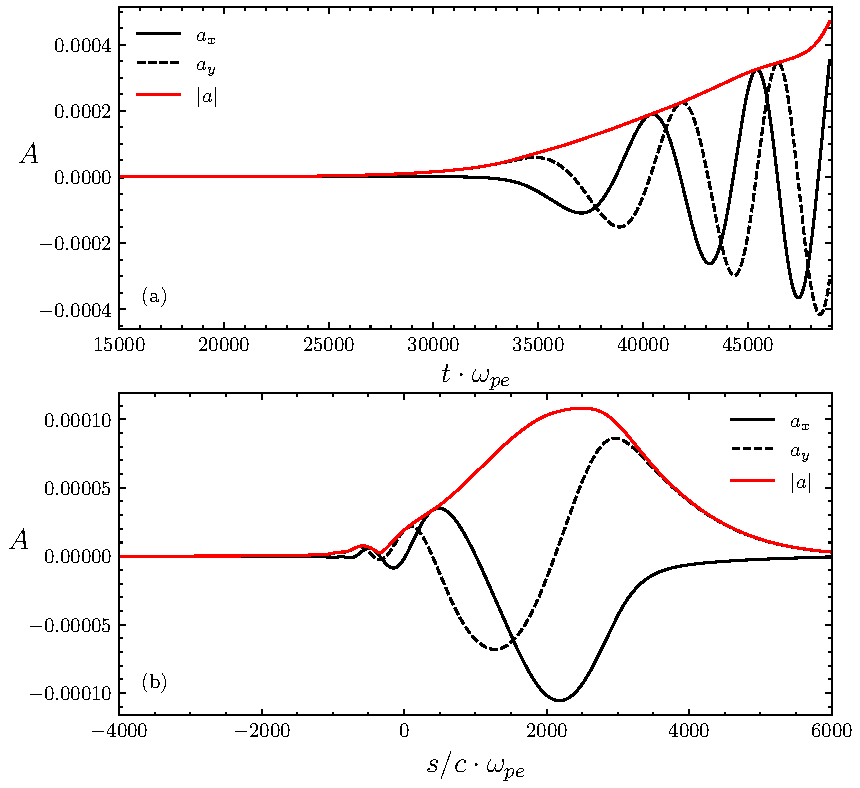
\includegraphics[scale=0.5]{img/aanda.pdf}
    \caption{Variation of (a) $\omega_{ce}$ and (b) $\Pi$ along the dipole field line.  (c) Time evolution and (d) spatial distribution of the orthogonal components of vector potential, $a_x$ and $a_y$, and the amplitude $|a|$ in the simulation.
    \label{fig.aanda}
    }
\end{figure}

The phase space trajectory can be obtained from the Hamilton's  equation,
\begin{equation}\label{eq.lab_eq}
    \begin{aligned}
        \frac{d\Omega}{dt} &= - \sqrt{2\omega_{ce}(s)\mu(s)} {\Im} (a(s,t)\cdot e^{-\imath \xi}) - \frac{\omega^2_{b}}{k_l^2(s)} \alpha
        \\
        \frac{d\xi}{dt} &= k_l^2(s) \Omega +\sqrt{\frac{\omega_{ce}(s)}{2\mu(s)}} {\Re}(a(s,t)\cdot e^{-\imath \xi})
    \end{aligned}
\end{equation}
where $\Im$ denotes taking the imaginary part.
With the calculated wave fields  in the Vlasov simulation \cite{zheng2024}, we solve the  equations of motion Eq. (\ref{eq.lab_eq}) using time-adaptive Runge-Kutta method. 
Then we push the resonant particle along the field line according to their characteristic lines in $s$-$\mathcal{J}$ space.
In the static resonance frame, the trapped particle does not have a closed phase space trajectory and their angle variable $\xi$ is shifting and matching with the wave phase $\delta \phi$ along its trajectory, as illustrated in Fig. \ref{fig.phaseflow}(a). This is in accordance with the phase locking condition \cite{tao_trap-release-amplify_2021}.
The varying phase $\delta \phi(s,t)$ also indicates the acceleration of trapped particles along $\Omega$ momentum dimension in phase space.
The momentum of the particle, as shown in Fig. \ref{fig.phaseflow}(b), is accelerating upwards along $\Omega$ dimension due to the rising tone frequency chirping.

\begin{figure}
    \centering
    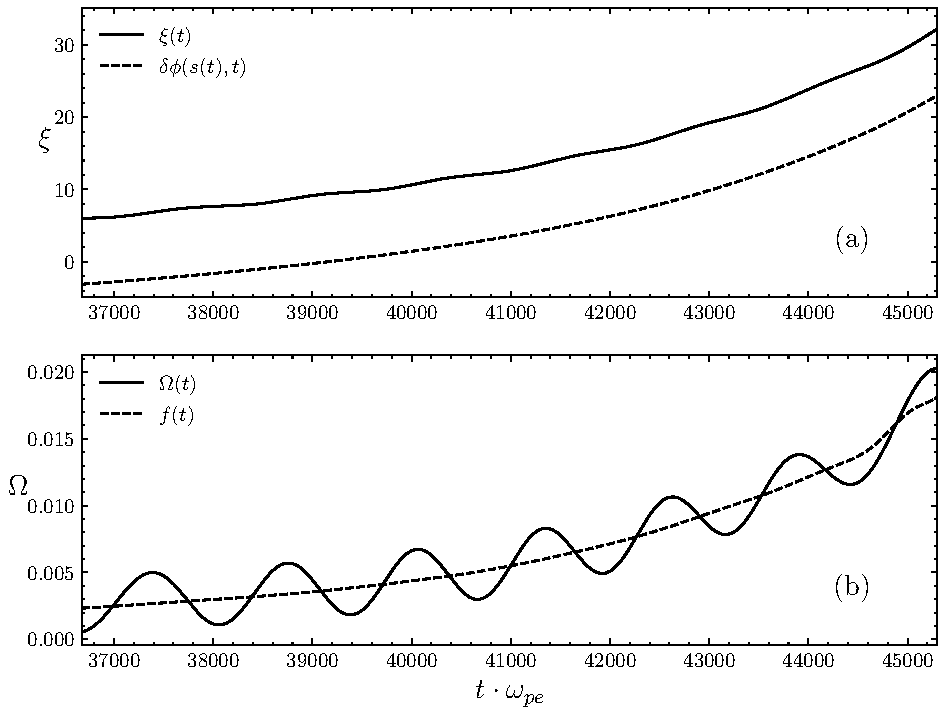
\includegraphics[scale=0.5]{img/phaseflow.pdf}
    \caption{
    (a) Typical variation of angle coordinate $\xi$ of a test particle and the  wave phase $\delta \phi$ along its trajectory.  (b) Particle momentum $\Omega$ versus time. The dashed line denotes Eq. (\ref{eq.ft}).
    \label{fig.phaseflow}
    }
\end{figure}

\begin{figure}
     \centering
     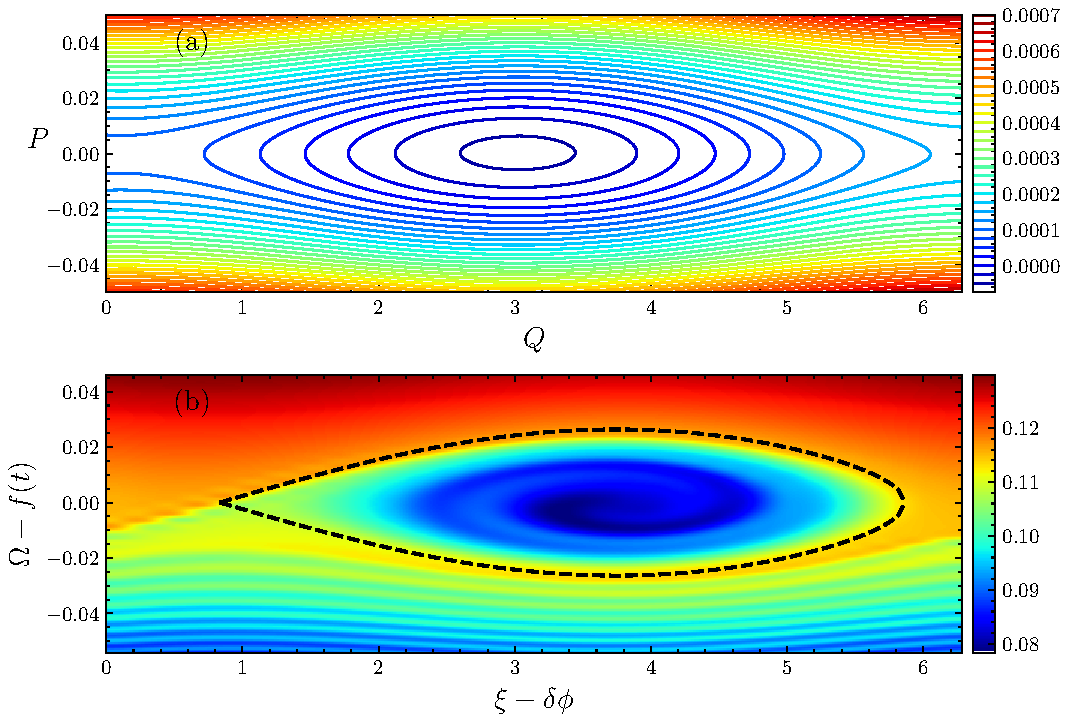
\includegraphics[scale=0.5]{img/Ham_and_f.pdf}
     \caption{(a)  
     Contour plot of  Hamiltonian 
Eq.~(\ref{eq.H_frame}) at $s\simeq2106c/\omega_{pe}$ and $t\simeq41564\omega_{pe}^{-1}$. 
 (b) Shifted phase space hole from the Vlasov simulation. The dashed line denotes the boundary of the hole obtained from Eq. (\ref{eq.bound}).
     \label{fig.hole}
     }
 \end{figure}

Since the wave phase $\delta \phi$ can be calculated from the Vlasov simulation
 \cite{zheng2024}, we can construct a canonical transformation to shift the static resonance frame to the real-time resonance frame.
The new canonical variables take the form \cite{berk1999},
\begin{equation}\label{eq.ct}
    \begin{aligned}
        Q &= \xi - \delta \phi(s(t),t)~,
        \\
        P & = \Omega - f(t)~,
    \end{aligned}
\end{equation}
where $f(t)$ is a time dependent function to be determined.
The canonical  transformation corresponds to a type-2 generating function \cite{goldstein2001}
\begin{equation}
    F_2(\xi,P,t) = (\xi - \delta \phi) \cdot P + \xi \cdot f(t)
\end{equation}
and the corresponding new Hamiltonian  is
\begin{equation}
    \begin{aligned}
        &  K^\prime = K + \frac{\partial F_2}{\partial t}
        \\
        & = \frac{k_l^2}{2}(P+f(t))^2 
        + \sqrt{2\omega_{ce}(\mathcal{J}+P+f(t)+\Pi)} \cdot |a|\cos Q 
        \\
        & + \left(\frac{1}{k_l}\left(\mathcal{J} - \frac{\Pi}{2} \frac{d\omega_{ce}}{ds}\right)  +\frac{d f(t)}{d t} \right)\cdot(Q + \delta \phi)  - \frac{d \delta \phi}{d t} P ~. 
        \end{aligned}
\end{equation}
In addition,  the first order term with respect to $P$  should be eliminated in the  Hamiltonian, which determines $f(t)$ as
\begin{equation}\label{eq.ft}
    \begin{aligned}
    f(t) & = \frac{1}{k_l^2} \frac{d \delta \phi}{d t}  &= \frac{\delta \omega - v_r \delta k}{k_l^2}~.
    \end{aligned}
\end{equation} 
The total time derivative is evaluated along the particle trajectory, $d/dt = \partial/\partial t + v_r \partial /\partial s$ with $\delta \omega  \equiv \partial \delta \phi/\partial t$ and $\delta k  \equiv -\partial \delta \phi/\partial s$.
The expression Eq. (\ref{eq.ft}) agrees with the change of $\Omega$ in the test particle simulation shown in Fig. \ref{fig.phaseflow}(b).
For the derivative of $f(t)$, we only keep the term up to the first order, which gives
\begin{equation}
    \frac{d f(t)}{d t} \simeq \frac{1}{k_l^2}(\frac{\partial \delta \omega}{\partial t} + 2 v_r \frac{\partial \delta \omega}{\partial s} + \frac{3}{2}v_r\frac{\delta k}{k_l} \frac{d \omega_{ce}}{d s}  ).
\end{equation}
Finally, the new Hamiltonian becomes 
\begin{equation}\label{eq.H_frame}
    K^\prime = \frac{k_l^2 P^2}{2} + \frac{{\omega^2_{b}}}{k_l^2} \cos Q +\frac{{\omega^2_{b}}}{k_l^2} \alpha \cdot Q~.
\end{equation}
With the canonical  transformation,
the $\omega_{b}$
and  $\alpha$ take the new form: 
\begin{equation}\label{eq.wbnew}
    \frac{{\omega^2_{b}}}{k_l^2} = \sqrt{2\omega_{ce}(\mathcal{J}+P+f(t)+\Pi)}  |a|
\end{equation}
and 
\begin{equation}\label{eq.alpnew}
    \begin{aligned}
    \frac{{\omega^2_{b}}}{k_l^2}\alpha & = \frac{1}{k_l}\left(\mathcal{J} - \frac{\Pi}{2}\right) \frac{d\omega_{ce}}{ds} \\
    & + \frac{1}{k_l^2}\left(\frac{\partial \delta \omega}{\partial t} + 2 v_r \frac{\partial \delta \omega}{\partial s} + \frac{3}{2}v_r\frac{\delta k}{k_l} \frac{d \omega_{ce}}{d s}\right)~.
    \end{aligned}
\end{equation}
The modified parameter $\alpha$ now describe the frequency chirping and the background magnetic field inhomogeneity.
The additional terms in Eq. (\ref{eq.alpnew}) compared to Eq.~(\ref{eq.alpold}) are the first order correction related to the frequency chirping and wave number variation.
In Fig.~\ref{fig.hole}(a),
the closed area of the Hamiltonian contour Eq.~(\ref{eq.H_frame})
implies the region where the particles are trapped. 
In the Vlasov simulation
\cite{zheng2024},
the center of the hole moves upwards in the canonical momentum  
$\Omega$
in phase space.  
According to the canonical transformation in Eq.~(\ref{eq.ct}),  the  phase space hole  can be shifted back to the center region where $\Omega-f(t)\simeq 0$, as shown in Fig.~\ref{fig.hole}(b). 
The trapped region from the Hamiltonian  in the real-time resonance frame  matches well with the shifted phase space hole from the Vlasov simulation in both the shape and the location.

\begin{figure}
    \centering
    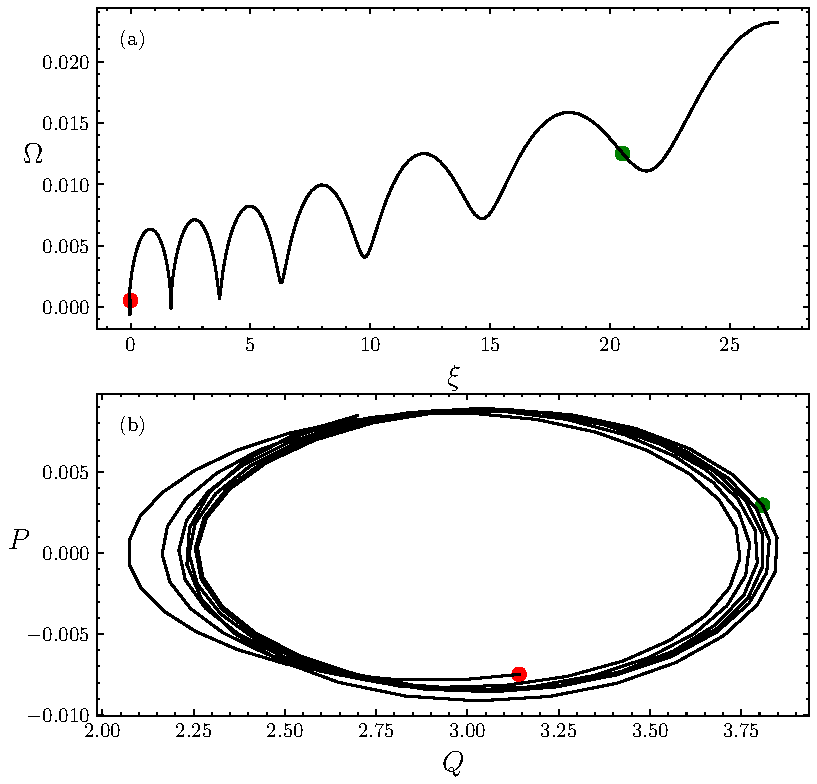
\includegraphics[scale=0.5]{img/Trajectory.pdf}
    \caption{Phase space trajectory of a test particle from $s \simeq 2107 c/\omega_{pe}$ at $t\simeq 36675 \omega_{pe}^{-1}$ 
    (red dots)
     to $s \simeq 205 c/\omega_{pe}$ at $t=45476 \omega_{pe}^{-1}$ 
    (green dots)
      in the (a) static  and  (b) real-time frames.  The corresponding enclosed phase space loop of a particle in the (c)  static and  (d) real-time  frames. 
    \label{fig.traj} 
    }
\end{figure}

 Using the new Hamiltonian, we can now consider  the particle dynamics in the real-time resonance frame
 where the Hamilton's equations have the same form as those in Eq.~(\ref{eq.lab_eq}) with the replacement of $\xi$ to $Q$ and $\Omega$ to $P$ and applying the new definition of ${\omega_{b}}$ and $\alpha$  in Eqs.~(\ref{eq.wbnew}) and (\ref{eq.alpnew}).
To show the differences, we choose a test particle initially at the resonance center and calculate its phase space trajectories in the different reference frames. In the static resonance frame, the particle suffers a rapid change in $\Omega$  for each bounce, as seen   in Fig. \ref{fig.traj}(a). In contrast, there exists only a slight change when we track the particle in the real-time resonance frame, as shown in Fig. \ref{fig.traj}(b), which demonstrates the effectiveness of the canonical transformation.


